\newpage
\subsection{[C] Giving editing permissions to a user}
To add a user from the list of people that have access to the list, just hover above the bubble, and click on the options button.

\begin{figure}[H]
  \centering 
  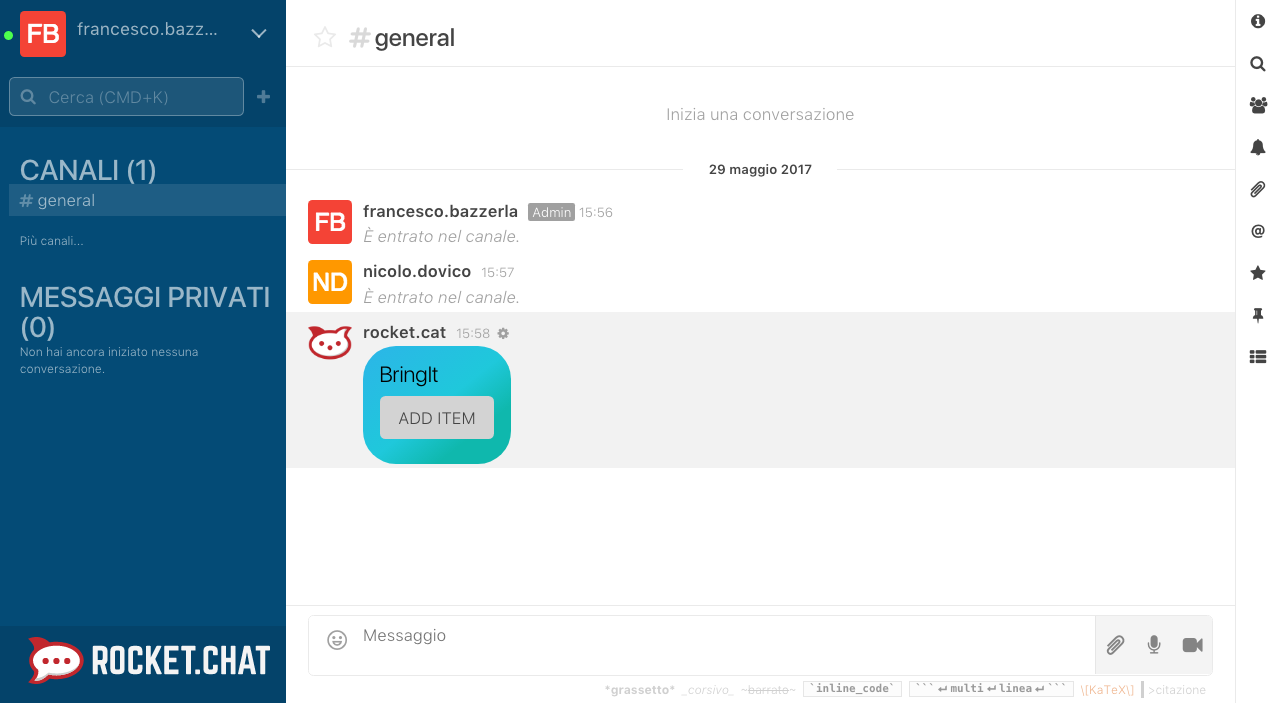
\includegraphics[width=\textwidth]{Sections/3-HowToUse/Images/bubble_options_button.png}
  \caption{Button to show the available list's actions.}
\end{figure}

Select then the button to add the permission to a user.

\begin{figure}[H]
  \centering 
  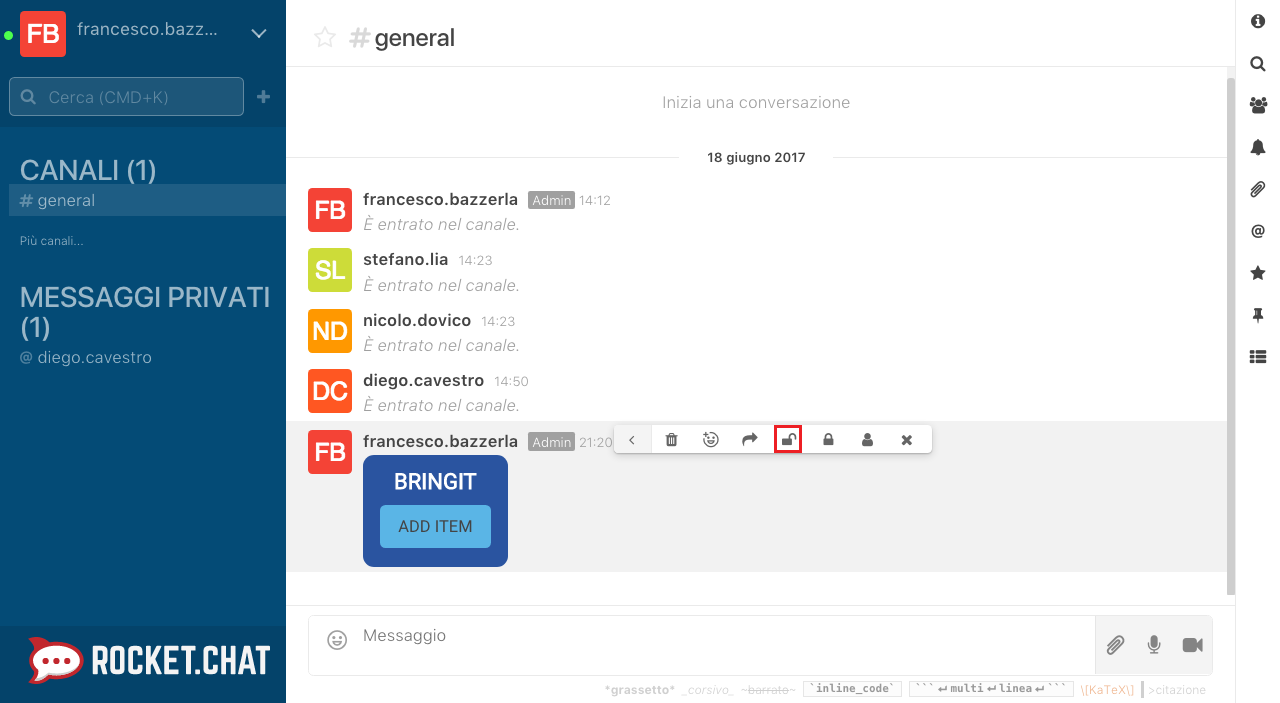
\includegraphics[width=\textwidth]{Sections/3-HowToUse/Images/bubble_option_permission_give.png}
  \caption{Button to remove the permissions of a user.}
\end{figure}

From the popup that opens, select the user(s) you want to add the permission to, and then click on "Ok".

\begin{figure}[H]
  \centering 
  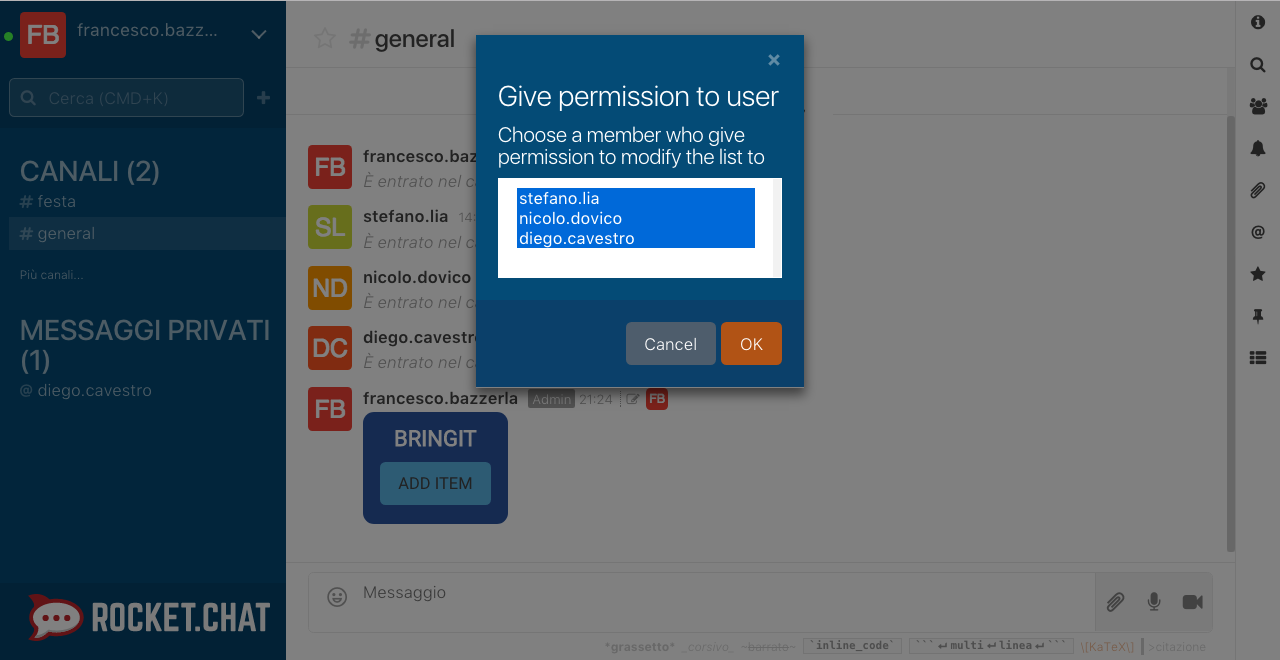
\includegraphics[width=\textwidth]{Sections/3-HowToUse/Images/popup_permission_give.png}
  \caption{Popup to remove the permissions of a user.}
\end{figure}

Note that, if there are no users from which you can remove the permissions, an error will be shown.

\begin{figure}[H]
  \centering 
  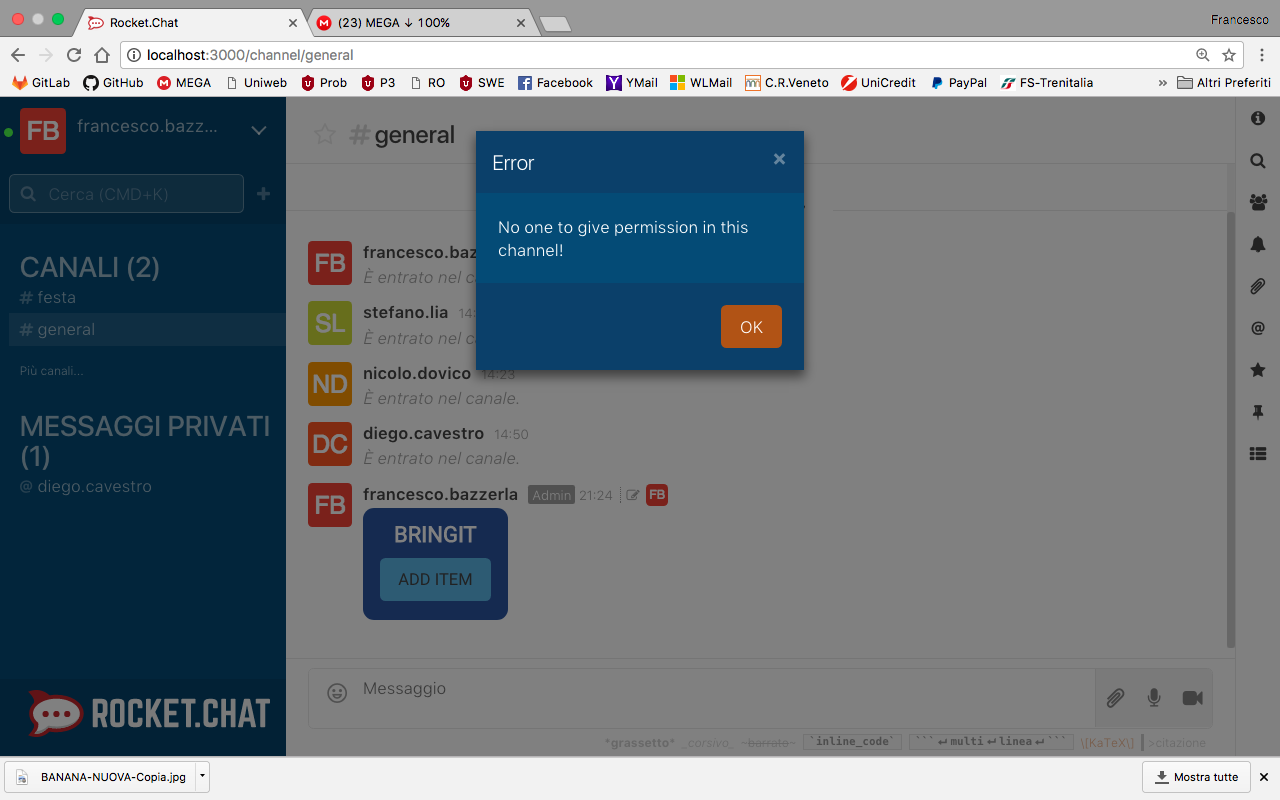
\includegraphics[width=\textwidth]{Sections/3-HowToUse/Images/popup_permission_give_error.png}
  \caption{Error shown if there are no people you can remove the permissions from.}
\end{figure}